\thispagestyle{cackithitoannone}
\pagestyle{cackithitoan}
\everymath{\color{cackithi}}
\graphicspath{{../cackithi/pic/}}
\begingroup
\AddToShipoutPicture*{\put(0,616){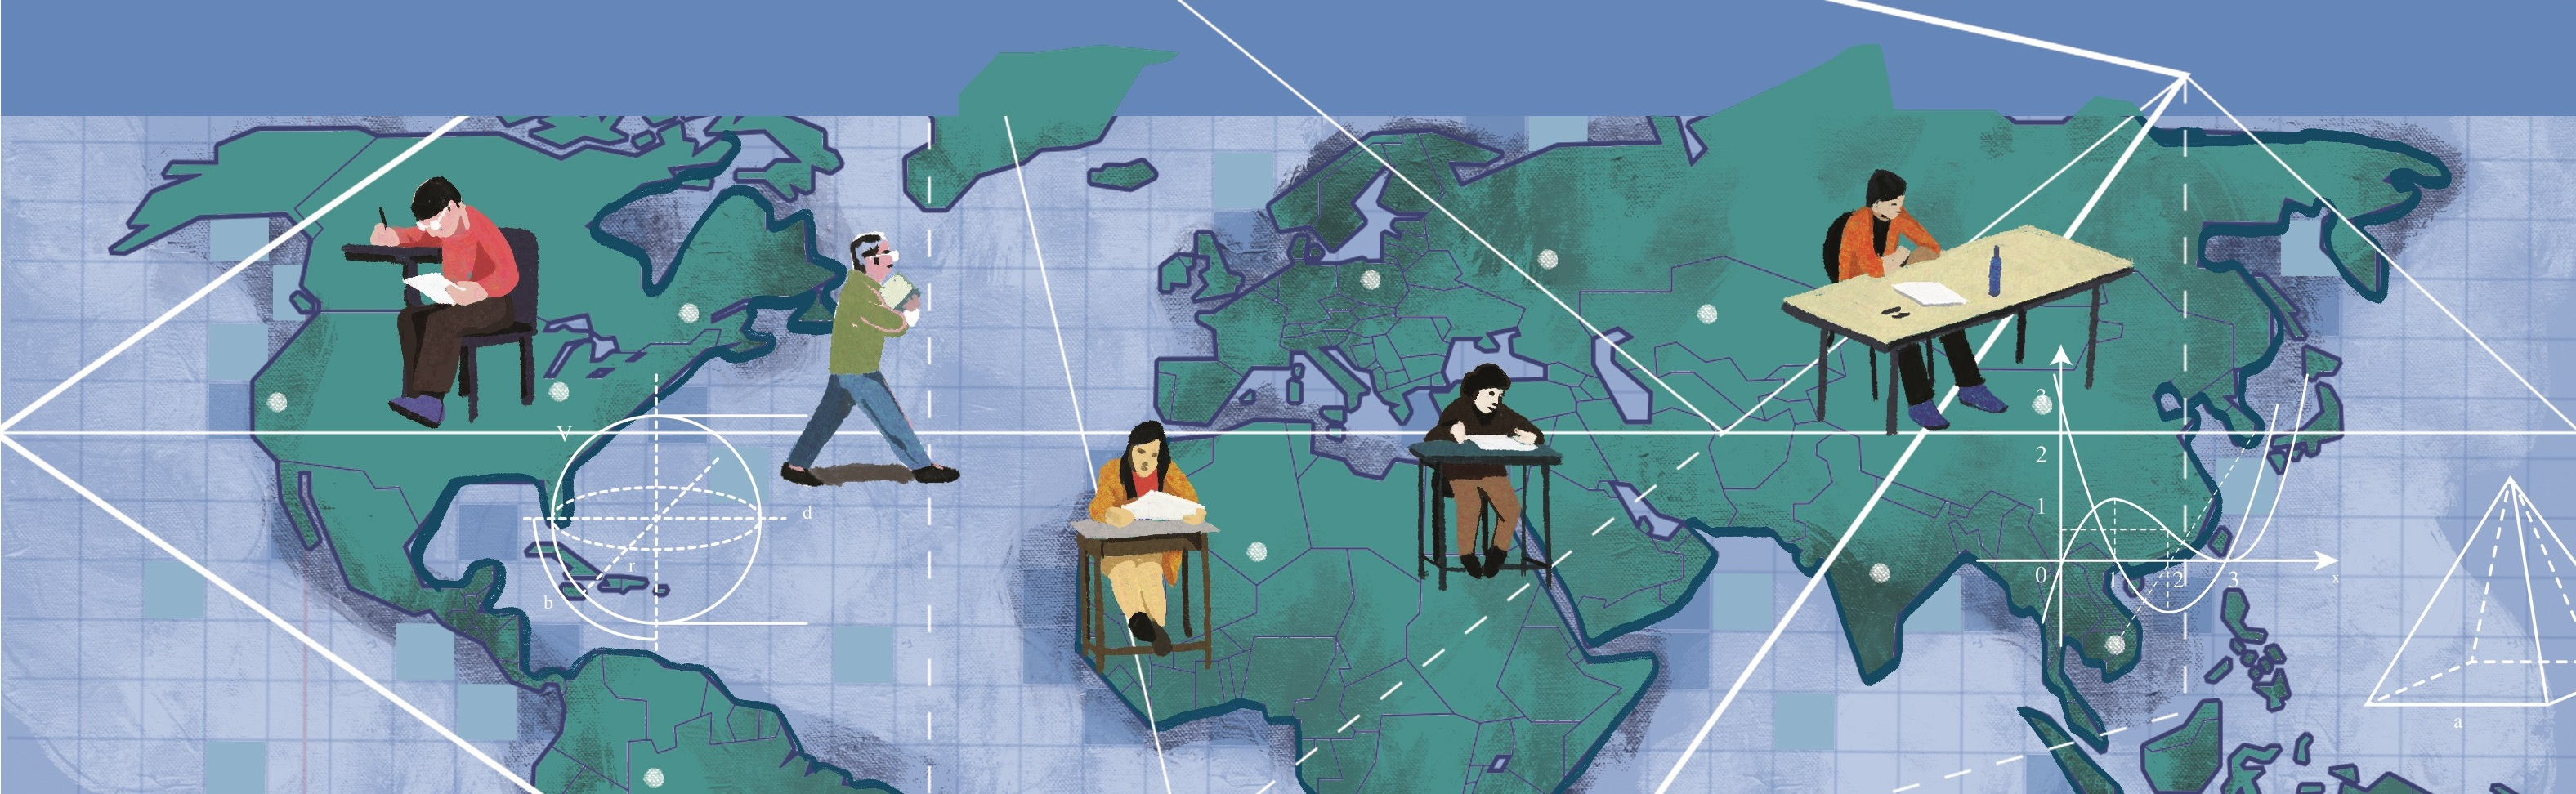
\includegraphics[width=19.3cm]{../bannercackithi}}}
\AddToShipoutPicture*{\put(100,555){
\includegraphics[scale=1]{../tieude.pdf}}}
\centering
\endgroup
\vspace*{150pt}

\begin{multicols}{2}
	Kỳ thi chọn học sinh giỏi quốc gia môn Toán THPT năm học $2022-2023$ được diễn ra trong hai ngày $24$ và $25/2/2023$ với tổng cộng $4{.}589$ thí sinh tham gia dự thi. Kết quả kỳ thi được công bố vào chiều tối ngày $13/3/2023$. Trong bài viết này, chúng tôi xin đưa ra một số tổng kết, đánh giá và bình luận về đề thi và kết quả của kỳ thi năm nay.
	\vskip 0.1cm
	\textbf{Về đề thi}
	\vskip 0.1cm
	Đề thi năm nay vẫn giữ ổn định cấu trúc đề thi HSG quốc gia môn toán từ gần $15$ năm nay, tức là $2$ ngày với ngày một có bốn bài, mỗi bài $5$ điểm và ngày hai có ba bài, số điểm tương ứng là $6$, $7$, $7$.
	\vskip 0.1cm 
	Ngày thứ nhất bốn bài toán lần lượt thuộc các phân môn: giải tích, số học, đại số và hình học. Bài toán giải tích là một bài toán thuộc chủ đề quen thuộc: giới hạn dãy số. Ý đầu ở mức căn bản sử dụng tính chất dãy đơn điệu và bị chặn thì có giới hạn, còn ý sau liên quan đến khảo sát dãy số ở dạng tích bằng cách logarit hóa. Việc sử dụng phép thế lượng giác chỉ giúp nhìn ra vấn đề nhanh hơn và giải gọn hơn chứ không phải là cách giải tiên quyết. Có thể đánh giá đây là bài dễ nhất của ngày thứ nhất cũng là bài dễ nhất của cả hai ngày. 
	\vskip 0.1cm
	Ở Bài $2$, bài số học, thì ý đầu là một ý hoàn toàn đại số và rất cơ bản, chúng ta có thể tìm được công thức tổng quát của dãy số một cách dễ dàng. Phần chính của bài toán này là ý sau (không liên quan gì đến ý đầu). Yêu cầu bài toán được phát biểu khá thú vị, thoạt nhìn thì có vẻ rất “khủng” nhưng nếu xem kỹ về bản chất thì khá đơn giản, chỉ dùng đến nguyên lý Dirichlet và tính tuần hoàn của số dư của dãy truy hồi nguyên. 
	\vskip 0.1cm
	Bài $3$ là một bài về bất đẳng thức ba biến có điều kiện, có thể nói là có dạng khá quen thuộc. Hướng đi tự nhiên nhất của bài này là chuẩn hóa rồi đưa về một biến (cụ thể là biến $r = abc$). Như vậy, xét về độ khó thì bài $3$ nhẹ nhàng hơn Bài $2$ cả về phát biểu (rất dễ hiểu), hướng đi và kỹ thuật.  
	\vskip 0.1cm
	Bài $4$ là một bài toán hình học có hai ý gần như độc lập. Ý đầu có điểm mấu chốt là có được $AKJH$ là hình bình hành rồi dùng tứ giác nội tiếp hoặc hàng điểm điều hoàn. Ý sau dùng tính chất của đường thẳng Simson và phép vị tự sẽ làm khá gọn. 
	\vskip 0.1cm
	Đánh giá sơ bộ cho đề thi ngày $1$ là đề khá dài, có nhiều ý, đặc biệt là các ý trong các Bài $2$ và $4$ hầu như không lên quan đến nhau. Các ý khó là $2b$ và $4a$, $4b$.
	\vskip 0.1cm 
	Đề thi ngày thứ hai gồm $3$ bài toán thuộc ba phân môn, lần lượt là: đại số, tổ hợp, hình học.
	\vskip 0.1cm
	Bài $5$ là một bài phương trình hàm có dạng giống (và cách giải cũng tương tự) với một bài toán trong IMO shortlist $2000$, khai thác tính toàn ánh và đơn ánh của phương trình hàm có biến nằm ngoài biểu thức hàm số. Không khó về mặt ý tưởng nhưng đây vẫn là một thách thức lớn cho thí sinh với những khó khăn kỹ thuật.   
	\vskip 0.1cm
	Bài $6$ là một bài toán tổ hợp về họ tập con khá quen thuộc sử dụng phương pháp đếm bằng hai cách. Dạng toán này đã xuất hiện nhiều, chỉ là với các tham số khác. Có lẽ khó khăn lớn nhất trong bài này là việc xây dựng ví dụ (nhất là trong tình huống các đánh giá đưa ra mới chỉ là các điều kiện cần). Phát biểu của bài toán này cũng hơi rối rắm và có lẽ điều đó cũng làm cho số thí sinh làm tốt bài này không nhiều.
	\vskip 0.1cm
	Bài $7$ là một bài toán hình học có cấu hình khá phức tạp với ý đầu là một bất đẳng thức hình học và ý sau yêu cầu chứng minh tính chất hình học thuần túy. Ý đầu có thể giải quyết khá gọn nếu biết một bổ đề quen thuộc sau: Cho góc xAy. Đường tròn $(I)$ tiếp xúc $Ax$, $Ay$ tại $B$, $C$. Đường tròn $(J)$ qua $A$ tiếp túc $(I)$ cắt $Ax$, $Ay$ tại $D$, $E$. Khi đó $AD + AE \ge BC$. Ý sau tuy có vẻ rối rắm nhưng lại có nhiều hướng để tiếp cận.
	\vskip 0.1cm
	So với ngày thứ nhất thì đề thi ngày thứ hai cân bằng hơn: Bài $6$ với hai ý $6a$, $6b$ khá nhẹ nhàng, Bài $5$ cũng có ý $5a$ cơ bản, còn lại các ý khó là $5b$, $6c$ và bài hình. 
	\vskip 0.1cm
	Về tổng thể đề thi năm nay được đánh giá là khó, dài với nhiều ý (hầu như bài nào cũng có ý $a$, $b$, thậm chí $c$), hơi nặng về kỹ thuật, phần hình học khá nặng với hai bài, bốn ý riêng biệt, cấu hình rất phức tạp và đều đặt ở vị trí bài cuối (và quả thật cũng là bài khó của từng ngày).
	\vskip 0.1cm
	\textbf{Về kết quả}
	\vskip 0.1cm
	Trước hết là điểm chuẩn. Dù đề thi năm nay được đánh giá là khá khó, dài và nhiều ý, nhưng điểm chuẩn không quá thấp như dự đoán ban đầu: KK -- $13{,}5$; Ba: $16{,}5$; Nhì: $20{,}5$; Nhất $27{,}5$ và điểm để dự thi chọn đội tuyển là $23$. 
	\vskip 0.1cm
	Kết quả tốt nhất thuộc về đội tuyển Hà Tĩnh với hai giải nhất, tám giải nhì. Trong đó có em Trần Minh Hoàng, học sinh lớp $10$ chuyên Hà Tĩnh đạt thủ khoa với số điểm $32$ (với một đề thi có đến năm bài ở mức khó thì đây là một kết quả tuyệt vời đối với một bạn học sinh lớp $10$).
	\vskip 0.1cm
	Tiếp theo là đội tuyển Phú Thọ với hai giải nhất, năm giải nhì, ba giải ba. Đội tuyển trường PTNK, ĐHQG--HCM vẫn giữ được phong độ với hai giải nhất, ba giải nhì, hai giải ba và hai giải KK. 
	\vskip 0.1cm
	Ngoài ba đơn vị dẫn đầu có hai giải nhất, các đơn vị có giải nhất và cũng có kết quả tốt là: ĐHKHTN, ĐQGHN: một giải nhất, ba nhì, ba giải ba; Bắc Ninh: một giải nhất, hai giải nhì, năm giải ba; Hà Nội, một giải nhất, ba giải nhì, bốn giải ba, sáu giải KK; Hải Phòng: một giải nhất, ba giải nhì, hai giải ba, hai giải KK; Thừa Thiên Huế: một giải nhất, một giải ba, bốn giải KK.
	\vskip 0.1cm
	Đây đều là các đơn vị có truyền thống của VMO. Ở một góc nhìn khác, VMO năm nay có những đơn vị có những thành tích vượt bậc so với chính mình như Sóc Trăng có một giải nhì, một giải ba, hai giải KK; Lâm Đồng có hai giải nhì, một giải ba, một giải KK; Điện Biên có hai giải ba, Trà Vinh có một giải nhì, Kiên Giang có một giải  ba, một giải KK. Đặc biệt, có hai bạn không phải là học sinh trường chuyên cũng đã xuất sắc đạt giải: một bạn học sinh THPT FPT Cần Thơ đạt giải ba và một bạn học sinh THCS \& THPT Đông Du Đăk lak đạt giải khuyến khích. 
	\vskip 0.1cm
	Cuối cùng xin được điểm qua về bản đồ TST năm nay. Với điểm chuẩn là $23$ có $48$ bạn đạt mốc điểm này, được phân bổ như sau: đông đảo nhất là Hà Tĩnh với tám bạn, tiếp đến là Phú Thọ với năm bạn. Năm đội mạnh tiếp theo, mỗi đội có ba học sinh gồm PTNK, ĐHQG--HCM; KHTN, ĐHQG--HN, ĐHSP HN, Hà Nội, Hải Phòng; các đội có hai thí sinh tham dự TST gồm Bắc Ninh, Nam Định, Nghệ An và Thanh Hóa. Cuối cùng là nhóm các đơn vị có một suất TST: Bà rịa -- Vũng Tàu, Bắc Giang, Đà Nẵng, Hải Dương, Hưng Yên, Lâm Đồng, Quảng Bình, Quảng Ngãi, Quảng Ninh, Tp HCM, Thừa Thiên -- Huế và Trà Vinh. $48$ em này sẽ cùng với bạn Phạm Việt Hưng, HCV IMO $2022$, tranh sáu suất dự IMO $2023$ tại Nhật Bản. 
	\vskip 0.1cm
	Trong các suất dự TST chúng tôi đặc biệt muốn nhắc tới hai suất của Trà Vinh và Lâm Đồng. Với Trà Vinh, có lẽ đây là suất TST đầu tiên còn với Lâm Đồng thì điều đặc biệt là suất TST này thuộc về học sinh trường chuyên Bảo Lộc, một trường chuyên thứ hai trong tỉnh mới được thành lập sau này. Và bạn học sinh đạt giải nhì có điểm số rất cao, $27$ điểm, tức là chỉ thiếu tí chút là đạt giải nhất.
	\vskip 0.1cm
	Nói câu chuyện về các trường hợp FPT Cần Thơ, Đông Du Đak lak, Điện Biên, Kiên Giang, Sóc Trăng, Trà Vinh hay chuyên Bảo Lộc để thấy rằng ở đâu cũng có học sinh có tố chất tốt, chỉ cần có những người thầy tâm huyết, biết thổi vào học trò sự tự tin và niềm đam mê. Ở thời đại của Internet, đặc biệt với sự cởi mở của cộng đồng toán, các vấn đề về tài liệu, thông tin sẽ không còn là lợi thế của riêng ai, và, với hình thức học online, các bạn học sinh ở mọi miền đều có cơ hội được học với các thầy giáo, các chuyên gia giỏi. Cơ hội được học hỏi đồng đều hơn và cơ hội thành công cũng đồng đều hơn.
	\vskip 0.1cm
	\textbf{Một số bình luận và đề xuất}
	\vskip 0.1cm
	Trước hết là về đề thi. Với thời gian $180$ phút làm bài, đề thi như vậy là quá dài với quá nhiều ý, quá nhiều yêu cầu, đặc biệt là ở ngày thi thứ nhất. Đề thi học sinh giỏi đa số là những bài mới, đòi hỏi thí sinh phải có nhiều thời gian suy nghĩ, tìm hướng tiếp cận rồi mới đến giai đoạn xử lý kỹ thuật, rồi lại phải trình bày chặt chẽ. Và kỹ thuật cũng không đơn giản (trên thực tế, hai bài toán có hướng đi khá rõ ràng là bài bất đẳng thức và bài phương trình hàm đã gây rất nhiều khó khăn cho các bạn học sinh). Theo ý kiến của chúng tôi, nên hạn chế các đề toán có nhiều ý mà chỉ nên đưa ra yêu cầu xử lý trọn vẹn một vấn đề. Nếu bài toán có hai ý trở lên thì nhất thiết chúng phải liên quan đến nhau và ý đầu sẽ như một gợi ý cho ý sau.
	\vskip 0.1cm
	Một vấn đề nữa nên có sự thay đổi là số lượng bài của mỗi ngày. Hiện nay, với cấu trúc ($4+3$) thì ngày thứ nhất có bốn bài toán, mỗi bài được $5$ điểm còn ngày thứ hai có ba bài toán, mỗi bài được $6$ hoặc $7$ điểm. Rõ ràng ngày thứ nhất sẽ có nhiều áp lực hơn vì trên thực tế, độ khó của các bài toán của hai ngày không có sự chênh lệch đáng kể. Đã thế điểm số tối đa của mỗi bài ở ngày thứ nhất chỉ là $5$ điểm (có thể tưởng tượng lấy được $5$ điểm ở bài $2$ hay bài $4$ khó thế nào). Vì vậy, chúng tôi đề xuất nên quay lại định dạng ba bài mỗi ngày như giai đoạn trước năm $2007$, cũng là một định dạng quen thuộc của nhiều kỳ thi toán trên thế giới. Với định dạng sáu bài thì trong hai ngày như vậy, phân bổ cho mỗi phân môn một bài và một bài ở dạng kiến thức tổng hợp. Như vậy sẽ đều hơn thay vì hơi nặng về hình học và đại số như hiện nay. 
	\vskip 0.1cm
	Cuối cùng, để tiếp nối ý đã trình bày ở cuối phần $2$, chúng tôi đề xuất nên triển khai mạnh hơn nữa các hoạt động dạy, bồi dưỡng chung cho các đối tượng học sinh (như các hoạt động trường hè, trường đông) để tạo cơ hội đồng đều cho các thí sinh. Việc tổ chức này sẽ được điều phối chung về chuyên môn bởi một Hội đồng chuyên môn (có thể là sự phối hợp giữa Bộ giáo dục, Hội toán học Việt Nam và Viện toán học) và các BTC địa phương lo các vấn đề hậu cần (hình thành các cụm). 
	\vskip 0.1cm
	Sau khi hình thành được các cụm để triển khai việc học tập, bồi dưỡng chung, có thể hướng đến việc tổ chức thi theo cụm với những hình thức sinh hoạt chuyên môn bổ ích như sửa bài thi, chia sẻ kinh nghiệm dạy và học toán, nghe các bài giảng đại chúng về toán học. Việc tổ chức thi cụm cũng giúp xóa tan những lăn tăn không đáng có về tính trung thực, nghiêm túc của kỳ thi, một điều luôn rất được coi trọng trong các kỳ thi tuyển chọn tài năng. 
	\vskip 0.1cm
	\textbf{Đề thi chọn học sinh giỏi Quốc gia THPT năm học} $2022-2023$
	\vskip 0.1cm
	\textbf{Bài} $\pmb{1}$ ($5{,}0$ điểm) Xét dãy số $\left(a_n\right)$ thỏa mãn $a_1 = \dfrac{1}{2}, a_{n+1} = \sqrt[3]{3a_{n+1} - a_n}$ và $0 \le a_n \le 1$, với mọi $n \ge 1$.
	\vskip 0.1cm
	$a)$ Chứng minh rằng dãy $(a_n)$ xác định duy nhất và có giới hạn hữu hạn.
	\vskip 0.1cm
	$b)$ Cho dãy số $\left(b_n\right)$ xác định bởi $b_n = (1+ 2a_1)\left(1 + 2^2a_2\right)\cdots\left(1 + 2^na_n\right)$ với mọi $n \ge 1$. Chứng minh rằng dãy $\left(b_n\right)$ có giới hạn hữu hạn.
	\vskip 0.1cm
	\textbf{Bài} $\pmb{2}$ ($5{,}0$ điểm) Cho các số nguyên $a,b,c, \alpha,\beta$ và dãy số $\left(u_n\right)$ xác định bởi 
	\begin{align*}
		u_1 = \alpha, u_2 = \beta, u_{n+2} = au_{n+1} + bu_n + c \text{ với mọi} n \ge 1.
	\end{align*}
	$a)$ Chứng minh rằng nếu $a=3, b = -2, c=-1$ thì có vô số cặp số nguyên $\left(\alpha, \beta\right)$ để $u_{2023} = 2^{2022}$.
	\vskip 0.1cm
	$b)$ Chứng minh rằng tồn tại số nguyên dương $n_0$ sao cho có duy nhất một trong hai khẳng định sau là đúng:
	\vskip 0.1cm
	$i)$ Có vô số số nguyên dương $m$ để $u_{n_0}u_{n_0+1}\cdots u_{n_0 + m}$ chia hết cho $7^{2023}$  hoặc $17^{2023}$;
	$ii)$ Có vô số số nguyên dương $k$ để $u_{n_0}u_{n_0+1}\cdots u_{n_0 +k} -1$ chia hết cho $2023$.
	\vskip 0.1cm
	\textbf{Bài} $\pmb{3}$ ($5{,}0$ điểm) Tìm ssoos thực dương $k$ lớn nhất sao cho bất đằng thức 
	\begin{align*}
		\frac{1}{kab + c^2} + \frac{1}{kbc + a^2} + \frac{1}{kca + b^2 } \ge \frac{k+3}{a^2 + b^2 + c^2}
	\end{align*}
	đúng với mọi bộ ba số thực dương $(a;b;c)$ thỏa mãn điều kiện $a^2 + b^2 + c^2 = 2 (ab+ bc + ca)$.
\end{multicols}
%\newpage
%\begingroup
%\AddToShipoutPicture*{\put(150,700){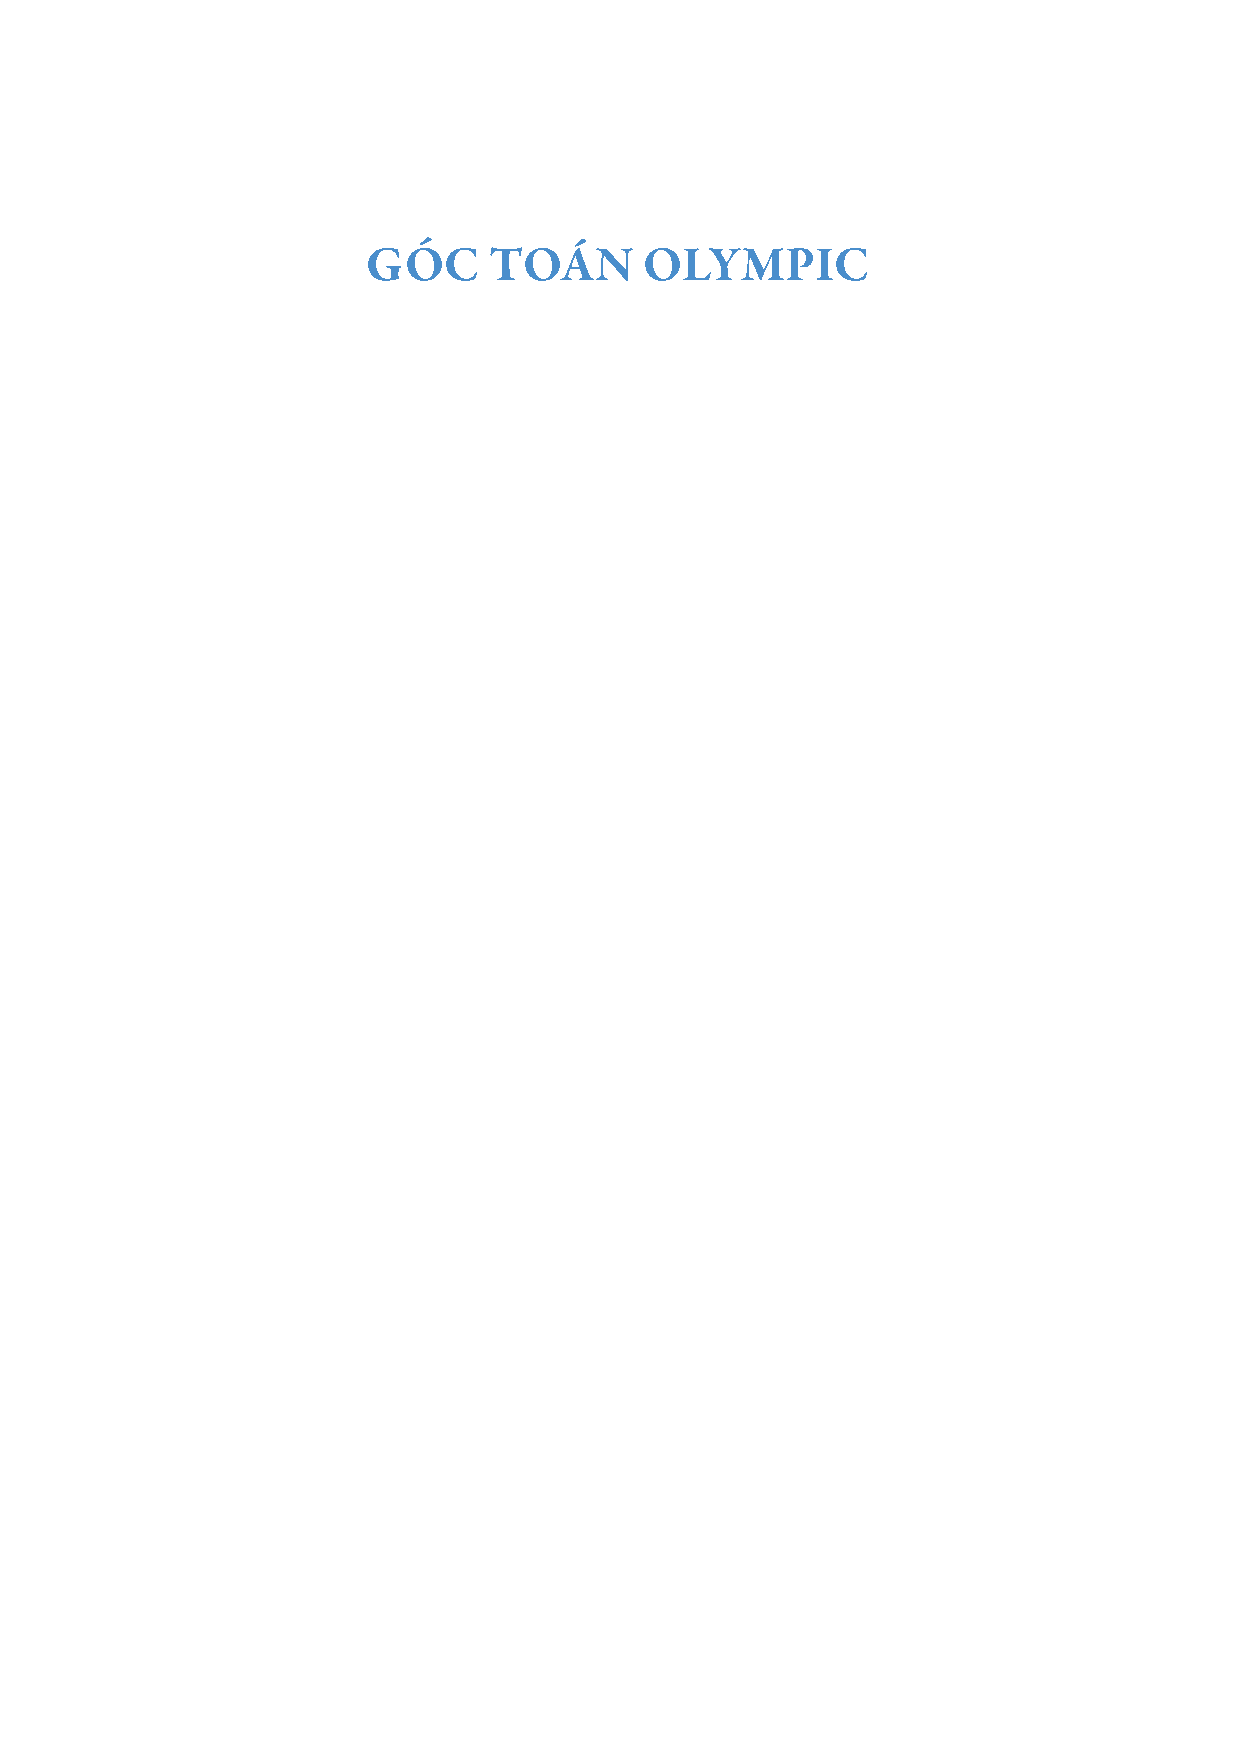
\includegraphics[scale=1]{../tieude1.pdf}}}
%\centering
%\endgroup
%\vspace*{1pt}
%
%\begin{multicols}{2}
%	Trong phần đầu chuyên mục, chúng tôi sẽ trình bày với các bạn lời giải của các bài toán trong kỳ thi Olympic Toán học vùng Cáp--ca năm học $2022$ (Caucasus Math Olympiad), đăng trong số báo tháng $12/2022$. 
%	\vskip 0.1cm
%%	\begin{figure}[H]
%%		\vspace*{-15pt}
%%		\centering
%%		\captionsetup{labelformat= empty, justification=centering}
%%		
\includegraphics[width= 0.85\linewidth]{gocolympic}
%%		\vspace*{-15pt}
%%	\end{figure}
%	{\bf\color{cackithi} OC$\pmb{28.}$} Cho trước các số nguyên dương $a, b, c$. Biết rằng $\dfrac{c}{b} = \dfrac{b}{a}$, và $b^2 - a - c + 1$ là số nguyên tố. Chứng minh rằng $\dfrac{a}{2}$ và $\dfrac{c}{2}$ là các số chính phương.
%	\vskip 0.1cm
%	\textit{Lời giải.} Từ đầu bài ta có $b^2=ac,$ từ đó thu được  $b^2 - a - c + 1=(a-1)(c-1)$ là số nguyên tố. Như vậy một trong hai số $a$ hoặc $c$ phải bằng $2$. Không mất tính tổng quát, giả sử $a=2,$ khi đó $b^2=2c$ như vậy $b$ là chẵn. Đặt $b=2k,$ thì $c=2k^2.$ Như vậy ta có điều cần chứng minh: $\dfrac{a}{2}=1$ và $\dfrac{c}{2}=k^2.$
%	\vskip 0.1cm
%	{\bf\color{cackithi} OC$\pmb{29.}$} Cho hình bình hành $ABCD$, các điểm $E$ và $F$ lần lượt nằm trên các đoạn $AD$ và $CD$ sao cho $\angle BCE = \angle BAF$. Các điểm $K$ và $L$ lần lượt nằm trên các đoạn $AD$ và $CD$ sao cho $AK = ED$ và $CL = FD.$ Chứng minh rằng $\angle BKD = \angle BLD.$
%	\begin{figure}[H]
%		\vspace*{-10pt}
%		\centering
%		\captionsetup{labelformat= empty, justification=centering}
%		\begin{tikzpicture}[cackithi,scale=1]
%			\draw [shift={(6,3)},fill=cackithi,fill opacity=0.10000000149011612] (0,0) -- (180:0.33403201021243345) arc (180:225:0.33403201021243345) -- cycle;
%			\draw [shift={(0,0)},fill=cackithi,fill opacity=0.10000000149011612] (0,0) -- (11.309932474020219:0.33403201021243345) arc (11.309932474020219:56.309932474020215:0.33403201021243345) -- cycle;
%			\draw  (0,0)-- (2,3);
%			\draw  (2,3)-- (6,3);
%			\draw  (6,3)-- (3,0);
%			\draw  (0,0)-- (4.615384615384616,0.9230769230769236);
%			\draw  (2,3)-- (5.384615384615384,2.0769230769230758);
%			\draw  (0,0)-- (1,0);
%			\draw  (0.5,0.10020960306372992) -- (0.5,-0.10020960306372992);
%			\draw  (1,0)-- (3,0);
%			\draw  (3,0)-- (4,0);
%			\draw  (3.5,0.10020960306372992) -- (3.5,-0.10020960306372992);
%			\draw  (4,0)-- (4.615384615384616,0.9230769230769236);
%			\draw  (4.201151925266359,0.4823833189696255) -- (4.36791078471567,0.3712107460034184);
%			\draw  (4.2474738306689455,0.5518661770735044) -- (4.414232690118257,0.44069360410729735);
%			\draw  (4.615384615384616,0.9230769230769236)-- (5.384615384615384,2.0769230769230758);
%			\draw  (5.384615384615384,2.0769230769230758)-- (6,3);
%			\draw  (5.585767309881747,2.559306395892701) -- (5.752526169331055,2.4481338229264944);
%			\draw  (5.632089215284331,2.6287892539965805) -- (5.79884807473364,2.5176166810303733);
%			\draw [fill=white] (0,0) circle (1.5pt);
%			\draw (-0.22221545793430705,-0.21615426902148865) node {$A$};
%			\draw [fill=white] (2,3) circle (1.5pt);
%			\draw (1.8988878069146455,3.4414962428046536) node {$B$};
%			\draw [fill=white] (6,3) circle (1.5pt);
%			\draw (6.141094336612552,3.357988240251545) node {$C$};
%			\draw [fill=white] (4,0) circle (1.5pt);
%			\draw (4.003289471252977,-0.28296067106397527) node {$D$};
%			\draw [fill=white] (3,0) circle (1.5pt);
%			\draw (2.9510886390838107,-0.2662590705533536) node {$E$};
%			\draw [fill=white] (1,0) circle (1.5pt);
%			\draw (0.9970013793410751,-0.249557470042732) node {$K$};
%			\draw [fill=white] (4.615384615384616,0.9230769230769236) circle (1.5pt);
%			\draw (4.888474298315926,0.9863609677432703) node {$F$};
%			\draw [fill=white] (5.384615384615384,2.0769230769230758) circle (1.5pt);
%			\draw (5.706852723336388,2.055263400423056) node {$L$};
%		\end{tikzpicture}
%		\vspace*{-10pt}
%	\end{figure}
%	\textit{Lời giải.}
%	Từ giả thiết, ta có
%	\begin{align*}
%		\angle ECD&= \angle BCD - \angle BCE \\
%		&= \angle BAD - \angle BAF = \angle FAD.
%	\end{align*}
%	Ta thu được hai tam giác $ECD$ và $FAD$ đồng dạng và từ đó có đẳng thức $\dfrac{ED}{FD} = \dfrac{DC}{DA}.$ Mặt khác ta có $\dfrac{ED}{FD} = \dfrac{AK}{CL}$ và $\dfrac{DC}{DA}=\dfrac{AB}{CB}.$ Do đó ta nhận được $\dfrac{AK}{CL}=\dfrac{AB}{CB},$  suy ra hai tam giác $AKB$ và $CLB$ đồng dạng. 
%	\vskip 0.1cm
%	Như vậy, ta có $\angle AKB=\angle CLB$ do đó nhận được   $\angle BKD = \angle BLD.$
%	\vskip 0.1cm
%	{\bf\color{cackithi} OC$\pmb{30.}$} Peter viết ra $21$ số nguyên dương đôi một phân biệt, mỗi số không lớn hơn $10^6$. Đối với mỗi cặp số $(a, b)$ được Peter viết ra, Nick  viết  số
%	\begin{align*}
%		F(a, b) = a + b - \gcd (a, b)
%	\end{align*}
%	trên mảnh giấy của mình (ở đây $\gcd$ ký hiệu ước chung lớn nhất). 
%	\vskip 0.1cm
%	Chứng minh rằng một trong những số mà Nick viết khác với tất cả những  số mà Peter viết. 
%	\vskip 0.1cm
%	\textit{Lời giải.} Ta chứng minh bằng phản chứng. Giả sử mọi số mà Nick viết ra đều trùng với một trong các số mà Peter đã viết. Ta xếp các số Peter viết theo thứ tự tăng dần:
%	\begin{align*}
%		a_1 < a_2 < \cdots < a_{20} < a_{21}.
%	\end{align*}
%	Khi đó, do $\gcd (a_{20}, a_{21}) \le a_{20},$ ta có  $F(a_{20}, a_{21}) = a_{20} + a_{21} - \gcd (a_{20}, a_{21})\ge a_{21}.$ Như vậy dấu bằng phải xảy ra, tức là $\gcd (a_{20}, a_{21}) = a_{20}$ ta suy ra $a_{21}$ là bội của $a_{20}.$
%	\vskip 0.1cm
%	Ta sẽ chứng minh $a_{k+1}$ là bội của $a_k$ với mọi $k=1, \cdots, 20.$ Thật vậy, với $k=20$ điều này đúng. Giả sử trái lại, gọi $k<20$ là số lớn nhất mà $a_{k+1}$ không là bội của $a_k.$ Khi đó, lý luận như trên ta có $F(a_{k}, a_{k+1})>a_{k+1}$. Mặt khác, do $a_{k+2}$ là bội của $a_{k+1},$ ta có 
%	\begin{align*}
%		F(a_{k}, a_{k+1}) &= a_{k} + a_{k+1} - \gcd (a_{k}, a_{k+1})\\
%		&<  a_{k} + a_{k+1}< 2a_{k+1}\le a_{k+2}.
%	\end{align*}
%	Như vậy $F(a_{k}, a_{k+1})$ không trùng với bất kỳ số nào Peter viết ra, điều này mâu thuẫn với giả thiết phản chứng. Vậy ta chứng minh được $a_{k+1}$ là bội của $a_k$ với mọi $k=1, \cdots, 20.$
%	\vskip 0.1cm
%	Từ đây ta có
%	\begin{align*}
%		a_{21}&\ge 2a_{20} \ge 2^2 a_{19} \ge \cdots \ge 2^{19}a_2 \ge 2^{20}a_1\\
%		&\ge 2^{20}>10^6.
%	\end{align*}
%	Điều này trái với giả thiết, như vậy ta có điều cần chứng minh. 
%	\vskip 0.1cm
%	Trong phần cuối của chuyên mục kỳ này, chúng tôi sẽ giới thiệu với bạn đọc ba bài toán trong kỳ thi toán của Đan Mạch mang tên nhà toán học Georg Mohr. Các bài toán này phù hợp với trình độ học sinh lớp $5-7$.
%	\vskip 0.1cm
%	{\bf\color{cackithi} OC$\pmb{37.}$} Một con ếch nhảy vào các số nguyên trên trục số. Nếu đang ở một số $n$ chẵn, bước tiếp theo nó sẽ nhảy đến số $\dfrac{n}{2}.$ Nếu đang ở một $n$ số lẻ, nó sẽ nhảy đến số $n + 5$. Tại một thời điểm nó nhảy vào số $25$. Hỏi trước đó $3$ bước nó có thể ở những vị trí nào?
%	\vskip 0.1cm
%	{\bf\color{cackithi} OC$\pmb{38.}$} Các số $1, 2, 3, \cdots, 16$  được đặt trong $16$ ô vuông xung quanh một bảng ô vuông cỡ $5\times 5$ như hình bên sao cho tổng của $5$ số trên mỗi cạnh của hình vuông là bằng nhau. 
%	Tổng nhỏ nhất có thể có của bốn số trong các ô vuông ở góc là bao nhiêu?
%	\begin{figure}[H]
%		\vspace*{-5pt}
%		\centering
%		\captionsetup{labelformat= empty, justification=centering}
%		\begin{tikzpicture}[scale=0.5,cackithi]
%			\draw (0,0) grid (5,5);
%			\draw[fill=white] (1,1) rectangle(4,4);
%		\end{tikzpicture}
%		\vspace*{-10pt}
%	\end{figure}
%	{\bf\color{cackithi} OC$\pmb{39.}$} Cho hình đa giác đều 9 cạnh $ABCDEFGHI$ như hình vẽ. Chứng minh rằng $AB + AC =AE.$
%	\begin{figure}[H]
%		\vspace*{-5pt}
%		\centering
%		\captionsetup{labelformat= empty, justification=centering}
%		\begin{tikzpicture}[cackithi,scale=0.5]
%			\draw  (1,2)-- (3,2);
%			\draw  (3,2)-- (4.532088886237956,3.2855752193730785);
%			\draw  (4.532088886237956,3.2855752193730785)-- (4.879385241571817,5.255190725397494);
%			\draw  (4.879385241571817,5.255190725397494)-- (3.879385241571817,6.9872415329663715);
%			\draw  (3.879385241571817,6.9872415329663715)-- (2,7.671281819617709);
%			\draw  (2,7.671281819617709)-- (0.12061475842818448,6.987241532966372);
%			\draw  (0.12061475842818448,6.987241532966372)-- (-0.8793852415718164,5.255190725397496);
%			\draw  (-0.8793852415718164,5.255190725397496)-- (-0.5320888862379562,3.28557521937308);
%			\draw  (-0.5320888862379562,3.28557521937308)-- (1,2);
%			\draw  (1,2)-- (4.532088886237956,3.2855752193730785);
%			\draw  (1,2)-- (3.879385241571817,6.9872415329663715);
%				\draw [fill=white] (1,2) circle (1.5pt);
%				\draw (0.7965821732136155,1.587828189189382) node {$A$};
%				\draw [fill=white] (3,2) circle (1.5pt);
%				\draw (3.1515078452112713,1.58212313902106253) node {$B$};
%				\draw [fill=white] (4.532088886237956,3.2855752193730785) circle (1.5pt);
%				\draw (4.955071097294682,3.2744802376984405) node {$C$};
%				\draw [fill=white] (4.879385241571817,5.255190725397494) circle (1.5pt);
%				\draw (5.222506308528359,5.4122851030580135) node {$D$};
%				\draw [fill=white] (3.879385241571817,6.9872415329663715) circle (1.5pt);
%				\draw (4.019991071763599,7.349670762290128) node {$E$};
%				\draw [fill=white] (2,7.671281819617709) circle (1.5pt);
%				\draw (2.0157990104889976,8.18475078782121) node {$F$};
%				\draw [fill=white] (0.12061475842818448,6.987241532966372) circle (1.5pt);
%				\draw (-0.13870745538119822,7.383073963311371) node {$G$};
%				\draw [fill=white] (-0.8793852415718164,5.255190725397496) circle (1.5pt);
%				\draw (-1.2243114885716069,5.345478701015527) node {$H$};
%				\draw [fill=white] (-0.5320888862379562,3.28557521937308) circle (1.5pt);
%				\draw (-0.8566666742742002,3.040657830549737) node {$I$};
%		\end{tikzpicture}
%		\vspace*{-5pt}
%	\end{figure}
%\end{multicols}
%\vspace*{-15pt}
%{\color{cackithi}\rule{1\linewidth}{0.1pt}}
%
%\vspace*{5pt}
%\centerline{\Large\textbf{\color{cackithi}LỜI GIẢI, ĐÁP ÁN}}
%
%\vspace*{-5pt}
%\begin{multicols}{2}
%	\textbf{\color{cackithi}Sự thật được làm rõ}
%	\vskip 0.1cm
%	Ta sẽ hỏi mỗi người trong số họ hai lần: ``Anh có phải là kẻ Nói dối không?"
%	\vskip 0.1cm
%	Kẻ Nói dối sẽ trả lời: ``không, không" và kẻ Thay đổi sẽ trả lời: ``có, không" hoặc ``không, có." Có ba câu trả lời có thể có từ kẻ Ranh mãnh.
%	\vskip 0.1cm
%	$1)$ ``Có, có." Khi đó, chúng ta ngay lập tức sẽ biết ai là ai.
%	\vskip 0.1cm
%	$2)$ ``Không, không." Khi  đó, chúng ta biết ngay ai là kẻ Thay đổi và câu trả lời nào trong số hai câu trả lời của anh ta là đúng. Chúng ta  đặt tiếp một câu hỏi cho Thay đổi: ``Anh ta có phải là kẻ Nói dối không?" và chỉ vào một trong hai người còn lại. Vì chúng ta đã biết liệu Thay đổi có trả lời đúng sự thật cho câu hỏi thứ ba hay không, nên chúng ta sẽ hiểu ngay ai trong số hai người là Nói dối, và do đó, ai trong số họ là kẻ Ranh mãnh.
%	\vskip 0.1cm
%	$3)$ ``Có, không" hoặc ``không, có." Khi đó, chúng ta  biết ngay kẻ Nói dối là ai. Hãy đặt câu hỏi cho kẻ  Nói dối: ``Anh ta có phải là một kẻ Ranh mãnh không?" và chỉ vào một trong hai người còn lại. Từ câu trả lời của người này, chúng ta sẽ tìm ra ai trong số hai người là Ranh mãnh, và do đó, ai trong số họ là kẻ Thay đổi.
%	\vskip 0.1cm
%	\textbf{\color{cackithi}Góc cờ}
%	\vskip 0.1cm
%	Hình $4$: $\pmb{1)}$ P$8/2$ T$5/7$\quad  $\pmb{2)}$ Tg$5-6$ T$7.9$\quad $\pmb{3)}$ T$3.5$ T$9.7$\quad $\pmb{4)}$ P$8-4$ T$3/5$\quad $\pmb{5)}$ C$5-4$ Tg$5.1$\quad $\pmb{6)}$ C$4.1$ T$5/3$\quad $\pmb{7)}$ C$4.1$ T$3.1$\quad $\pmb{8)}$ P$4-5$ T$7/5$\quad $\pmb{9)}$ P$5.7$ (Đen mất Tượng, Đỏ tiếp tục đưa Pháo về đáy dùng thủ đoạn tương tự bắt chết Tượng còn lại, Đỏ thắng)
%	\vskip 0.1cm
%	Hình $5$: $\pmb{1)}$ C$6.1$ T$9.7$\quad $\pmb{2)}$ P$5.3$ Ts$.9$\quad  $\pmb{3)}$ Tg$4/1$ T$9/7$\quad $\pmb{4)}$ Tg$4-5$ Ts$.9$\quad $\pmb{5)}$ Tg$5-6$ T$9/7$\quad $\pmb{6)}$ P$5-9$ S$4.5$\quad $\pmb{7)}$ Tg$6-5$ Ts$.9$\quad  $\pmb{8)}$ P$9-3$ T$7/5$\quad $\pmb{9)}$ P$3-5$ T$9/7$\quad $\pmb{10)}$ Tg$5-6$ T$7.9$\quad $\pmb{12)}$ C$6.1$ $(1-0)$.
%	\vskip 0.1 cm
%	\hfill (\textit{Xem tiếp trang} $45$.)
%\end{multicols}